\documentclass[a4paper,11pt]{article}

\usepackage[latin1,utf8]{inputenc}
\usepackage[T1]{fontenc}
\usepackage[french, francais]{babel}
\usepackage{fullpage}
\usepackage{url}

\usepackage{pgf}
\usepackage{tikz}
\usepackage{pgfgantt}
\usepackage{subcaption}
\usepackage{amsmath}
\usepackage{amssymb}
\usepackage{mathrsfs}
\usepackage{xcolor}
\usepackage{minted}
\usepackage{subcaption}

\newcommand{\Python}[1]{\mintinline{python}{#1}}

\newcommand{\carybe}[1]{ \textcolor{magenta}{#1}}

\title{Rapport projet M1 :\\Implémentation d'une résolution de l'équation de Vlasov}

\author{Carybe \bsc{Bégué}}

\begin{document}

\maketitle


\section{Résumé}

Lors de ce projet, j'ai implémenté une résolution de l'équation de Vlasov en Julia. J'ai été encadré par Nicolas Crouseilles et Erwan Faou de l'équipe Mingus de l'Inria de Rennes.

Mon code se base sur la notion de méta particules et l'hypothèse que la fonction de distribution de probabilité des particules est une somme de Dirac en espace et en vitesse. Les particules sont représentées en une dimension. 

Les différents paramètres sur lesquels l'utilisateur peut jouer sont :
\begin{itemize}
	\item \Python{nstep} le nombre d'itérations ;
	\item \Python{dt} le pas de temps ;
	\item \Python{L} la taille du domaine en espace (le domaine est en réalité un cercle). De \Python{L} est débuit \Python{kx} ;
	\item \Python{k} le paramètre du troncature du noyau (voir section \ref{noyau});
	\item \Python{np} le nombre de particules ;
	\item \Python{nx} le nombre de mailles pour le calcul de l'énergie électrique selon la méthode PIC (voir section \ref{energie PIC}) ;
	\item \Python{alpha} la perturbation initiale (voir section \ref{samples}).
\end{itemize}

La fonction \Python{run} renvoit :
\begin{itemize}
	\item \Python{energy_hamil_elec} l'intégrale de l'énergie électrique calculée selon la méthode Hamiltonienne (voir section \ref{energy hamil}) ;
	\item \Python{energy_pic} l'intégrale de l'énergie électrique calculée selon la méthode PIC (voir section \ref{energie PIC}) ;
	\item \Python{energy_elec_from_phi} l'intégrale de l'énergie électrique calculée à partir du potentiel électrique (voir section \ref{energy pot}) ;
	\item \Python{energy_tot} l'énergie totale du système ;
	\item \Python{anime} le gif représentant l'évolution des particules au cours du temps (généré par la suite par la commande \Python{gif(anime)}).
\end{itemize}

L'ensemble du code est disponible sur le git \url{https://github.com/Carybou/Projet-M1-PIC}. La fonction \Python{run} se trouve dans le fichier \Python{simul/main.jl}. À la fin du fichier, je propose une exécution de \Python{run} ainsi que l'affichage de l'énergie totale et du logarithme de l'énergie électrique calculée selon les 3 méthodes de la section \ref{energy}.

\section{Solution $\Delta u = f$}
\label{delta u}

On cherche à résoudre l'équation $\Delta u = f$ d'inconnue $u$, avec $\Delta u$ laplacien de u, dans $\mathcal{R}^d$.

$$
\begin{array}{rclr}

\Delta u &=& f \\

\sum\limits_{n=1}^d {\partial^2_ {x_n}} u(x) &=& f(x) \\

\sum\limits_{n=1}^d (ik_n)^2 \widehat{u}(k) &=& \widehat{f}(k) & \text{par transformée de Fourier} \\

-|k|^2  \widehat{u}(k) &=& \widehat{f}(k) & \text{si } \widehat{f}(0)=0 \\

\end{array}
$$

Notons $\mathcal{N} (x) = \sum\limits _{k \in \mathbb{Z}^{d*}} \frac{1}{|k|^2} e^{ik.x}$. En fourier $\widehat{\mathcal{N}}(k) = \frac{1}{|k|^2}$.

D'où :

$$
\begin{array}{rclr}

\widehat{u} (k) &=& - \mathcal{N}(k) \times \widehat{f} (k) \\

u(x) &=& - (\mathcal{N} \ast f) (x)

\end{array}
$$

\section{Application à Vlasov}

L'équation de Vlasov d'inconnue $f$, fonction de $x \in [0, L]$, $v$ et $t$ est :
$$
\partial_t f + v \partial_x f - \partial_ x \Phi \partial_v f = 0
$$

Avec : $\Delta \Phi [f](x,t) =  - \int f(x,v,t) dv +  \frac{1}{L} \int \int f(x, v , t) dx dv$, potentiel d'intéraction.

D'après la partie \ref{delta u}, $\Phi[f](x,t) = (\mathcal{N} \ast \int f(x,v,t)dv) (t)$, en supposant $\Delta \Phi [f]$ de moyenne nulle.

Soit $(X,V, \beta) = (X_k(t),V_k(t), \beta_k)_{k \in [\![ 1, N]\!]}$ une solution apporché de la fonction de distribution représentant $N$ méta particules de position à l'instant $t$ $X_k(t)$, de vitesse $V_k(t)$ et de masse donnée $\beta_k \in \mathbb{R^+}$. On a pour toutes méta particules $k$ :

$$
\left\lbrace
\begin{array}{rcl}

\frac{dX_k}{dt} &=& V_k \\ \\
\frac{dV_k}{dt} &=& - \partial_x \Phi(X_k, t) \\

\end{array} \right.
$$

Faisons l'hypothèse que $f^n(X,V) = \sum\limits_k \beta_k \delta_{X_k^n} \delta_{ V_k^n}$, avec $f^n(X,V) = f(X,V, t^n)$.

Ainsi :

$$
\begin{array}{rcl}

\Phi[f](x,t^n) &=& (\mathcal{N} \ast \int f(x,v,t^n)dv) (t^n) \\
	&=&  (\mathcal{N} \ast \int \sum\limits_k \beta_k \delta_{X_k^n} \delta_{ V_k^n}dv) (t^n) \\
	&=& (\mathcal{N} \ast \sum\limits_k \beta_k \delta_{X_k^n} \int \delta_{ V_k^n}dv) (t^n) \\
	&=& (\mathcal{N} \ast \sum\limits_k \beta_k \delta_{X_k^n}) (t^n) \\
	&=& \int \mathcal{N}(x-y) \sum\limits_k \beta_k \delta_{X_k^n}(y) dy \\
	&=& \sum\limits_k \beta_k  \int \mathcal{N}(x-y) \delta_{X_k^n}(y) dy \\
	&=& \sum\limits_k \beta_k  \mathcal{N}(x-X_k^n) \\

\end{array}
$$

Et ainsi : 
$$
\boxed{\frac{d V_k} {dt} = -\sum\limits_{l=1}^N \beta_l  \mathcal{N}'(X_k^n-X_l^n)}
$$

En discrétisant le temps, on considère à présent les instants $(t^0, t^1, \dots)$ d'intervalle $\Delta t$. Chaque méta particule est donc représenté par deux suites $(X_k^n, V_k^n)_{n \in \mathbb{N}}$.

$$
\left\lbrace
\begin{array}{rclr}

\frac{X_k^{n+1} - X_k^n}{\Delta t} &=& V_k^{n+1} & (1) \\ \\
\frac{V_k^{n+1} - V_k^n}{\Delta t} &=& - \sum\limits_{l = 1}^N \beta_l  \mathcal{N}'(X_k^n-X_l^n) & (2)\\

\end{array} \right.
$$

L'équation $(1)$ est implicite, pour résoudre ce système, il faut procéder en 2 deux temps :

$$
\Phi _ v ^{\Delta t} \left\lbrace
\begin{array}{rclr}

\frac{X_k^{n+1} - X_k^n}{\Delta t} &=& 0  \\ \\
\frac{V_k^{n+1} - V_k^n}{\Delta t} &=& - \sum\limits_{l = 1}^N \beta_l  \mathcal{N}'(X_k^n-X_l^n)\\

\end{array} \right.
$$

$$
\Phi _T ^{\Delta t}  \left\lbrace
\begin{array}{rclr}

\frac{X_k^{n+1} - X_k^n}{\Delta t} &=& V_k^{n+1} \\ \\
\frac{V_k^{n+1} - V_k^n}{\Delta t} &=& 0\\

\end{array} \right.
$$

On résoudre en premier le système $\Phi _v$ pour calculer $V_k^{n+1}$ puis le système $\Phi _t$ pour calculer $X_k^{n+1}$.

$$
(X_k^{n+1}, V_k^{n+1}) = (\Phi_T^{\Delta t} \circ \Phi_v^{\Delta t}) (X_k^{n}, V_k^{n})
$$

On peut résumer ces équations à un système Hamiltonien non cannonnique :

$$
H(X,V) = \frac{1}{2} \sum \limits_{k} \beta_k v_k^2 + \frac{1}{2} \sum \limits _{k, l} \beta_k \beta_l \mathcal{N}(x_k - x_l)
$$

Avec :
$$
\left\lbrace
\begin{array}{rcl}
	\dot{x_k} &=& \frac{1}{\beta_k} \partial_{v_k} H \\
	\dot{v_k} &=& - \frac{1}{\beta_k} \partial_{x_k} H \\

\end{array}
\right.
$$

\section{Échantillonage initial}
\label{samples}

Notre solution $f_0$ de l'équation de Vlasov au temps inital est :
$$
f_0(x,v,t) = \frac{1}{2 \pi} ( 1 + \alpha cos(k_x x))
 exp( - \frac{v^2}{2})
$$

avec $k_x = \frac{L}{2 \pi}$ avec $L$ la taille du domaine et $\alpha \in [0, 1[$ une petite perturbation. Notons que si $\alpha = 0$ alors $f_0$ est un solution stationnaire de l'équation de Vlasov. $k_x$ vaut environ $0.5$ et $\alpha << 1$ en général.

\paragraph{Échantillonage de $v$} 
La vitesse est simplement échantillonée selon une gaussienne centrée en 0 et d'écart-type 1.

\paragraph{Échantillonage de $x$}
La position des particules doit être échantillonée selon une densite $f_x(x) = ( 1 + \alpha cos(k_x x)$. Pour ce faire, on résout l'équation :
$$
\int_0^x (1 + \alpha cos(k_x y)) dy = x + \frac{\alpha}{k_x} sin(k_x x) = r
$$
avec $r \in [0, 1]$ choisi aléatoirement. Cette équation est résolue grâce à la méthode de Newton.

L'échantillonage est fait dans la fonction \Python{samples}.

\section{Calcul de la constante $C$}
\label{noyau}

Le calcul du noyau $\mathcal{N}$ dépend du domaine de définition $D$ choisi. Dans le cas où $D = \mathbb{R}$, on a bien $\mathcal{N} (x) = \sum\limits _{k \in \mathbb{Z}^{d*}} \frac{1}{|k|^2} e^{ik.x}$.

Cependant, on travaille ici dans $D=[0, L]$, ce qui implique l'ajout d'une constante multiplicative $C$ dans $\mathcal{N}$ \emph{ie.} $\mathcal{N} (x) = C \times \sum\limits _{k \in \mathbb{Z}^{d*}} \frac{1}{|k|^2} e^{ik.x}$.

Pour une fonction $g$ périodique de période $L$ et régulière, on a :
$$
g(x) = \sum\limits_{k \in \mathbb{Z}} e^{i\frac{2 \pi}{L} kx} \widehat{g}_k
$$
Avec :
$$
\widehat{g}_k = \frac{1}{L} \int_0 ^L e^{-i\frac{2 \pi}{L} kx} g(x) dx
$$

Pour déterminer $C$ on va chercher à définir $\Phi$ en fonction de $\rho$.
On veut résoudre :
$$
- \partial ^2 _x \Phi(x) = \rho (x)
$$
Avec : $\int _0 ^L \Phi(x) dx = 0$ et $\rho (x) = \sum\limits_{l=0} ^N \beta_l \delta(x - x_l)$

D'une part :
$$
\begin{array}{rcl}
- \partial ^2 _x \Phi(x) &=& - \partial ^2 _x \sum\limits_{k \in \mathbb{Z}} e^{i\frac{2 \pi}{L} kx} \widehat{\Phi}_k \\ \\
 &=& \sum\limits_{k \in \mathbb{Z}} \frac{4 \pi^2}{L^2}k^2 e^{i\frac{2 \pi}{L} kx} \widehat{\Phi}_k \\ \\
 &=& \sum\limits_{k \in \mathbb{Z}} e^{i\frac{2 \pi}{L} kx} (\frac{4 \pi^2}{L^2}k^2  \widehat{\Phi}_k) 
\end{array}
$$

D'autre part :
$$
\rho(x) = \sum\limits_{k \in \mathbb{Z}} e^{i\frac{2 \pi}{L} kx} \widehat{\rho}_k
$$
avec :
$$
\begin{array}{rcl}
\widehat{\rho}_k &=& \frac{1}{L} \int_0 ^L e^{-i\frac{2 \pi}{L} kx} \rho(x) dx \\
 &=& \frac{1}{L} \int_0 ^L e^{-i\frac{2 \pi}{L} kx} \sum\limits_{l=0} ^N \beta_l \delta(x - x_l) dx \\
 &=& \frac{1}{L} \sum\limits_{l=0} ^N \beta_l \int_0 ^L e^{-i\frac{2 \pi}{L} kx} \delta(x - x_l) dx \\
 &=& \frac{1}{L} \sum\limits_{l=0} ^N \beta_l e^{-i\frac{2 \pi}{L} kx_l} \\
\end{array}
$$

En identifiant $\widehat{\Phi}_k$ pour $k \in \mathbb{Z}^*$, on obtient :
$$
\begin{array}{rcl}
\widehat{\Phi}_k &=& \frac{L^2}{4 \pi^2 k^2} \widehat{\rho}_k \\
 &=& \frac{L}{4 \pi^2 k^2} \sum\limits_{l=0} ^N \beta_l e^{-i\frac{2 \pi}{L} kx_l}
\end{array}
$$

D'où, en supposant $\widehat{\Phi}_0 = 0$ : 
$$
\begin{array}{rcl}
\Phi(x) &=& \sum\limits_{k \in \mathbb{Z}^*} e^{i\frac{2 \pi}{L} kx} \frac{L}{4 \pi^2 k^2} \sum\limits_{l=0} ^N \beta_l e^{-i\frac{2 \pi}{L} kx_l} \\
 &=& \sum\limits_{k \in \mathbb{Z}^*} \sum\limits_{l=0} ^N \frac{L}{4 \pi^2 k^2} \beta_l e^{i\frac{2 \pi}{L} k( x -x_l)}
\end{array}
$$

On tronque la somme sur $k$ entre $-K$ et $K$ et on en débuit :
$$
\begin{array}{rcl}
\Phi(x) &=& \sum\limits_{\underset{k \neq 0}{k=-K}}^K e^{i\frac{2 \pi}{L} kx} \frac{L}{4 \pi^2 k^2} \sum\limits_{l=0} ^N \beta_l e^{-i\frac{2 \pi}{L} kx_l} \\
 &=& \sum\limits_{l=0} ^N \beta_l \sum\limits_{\underset{k \neq 0}{k=-K}}^K \frac{L}{4 \pi^2 k^2}  e^{i\frac{2 \pi}{L} k( x -x_l)}
\end{array}
$$

En identifiant $\mathcal{N}$, on obtient :
$$
\mathcal{N}(x) = \sum\limits_{\underset{k \neq 0}{k=-K}}^K \frac{L}{4 \pi^2 k^2}  e^{i\frac{2 \pi}{L} kx}
$$

Notons que lorsque $k=1$, l'équation à résoudre devient l'équation de Vlasov-HMF.

\section{Réécriture $\frac{dV_k}{dt}$}

Ainsi, en réinjcetant la formule de $\mathcal{N}$ dans $\frac{dV_m}{dt}$ on obtient :
$$
\begin{array}{rcl}
\frac{d V_m} {dt} &=& -\sum\limits_{l=1}^N \beta_l  \mathcal{N}'(X_m^n-X_l^n) \\
 &=& -\sum\limits_{l=1}^N \beta_l  \sum\limits_{\underset{k \neq 0}{k=-K}}^K i\frac{2 \pi}{L} k \frac{L}{4 \pi^2 k^2}  e^{i\frac{2 \pi}{L} k(X_m^n-X_l^n)} \\
 &=& -\sum\limits_{l=1}^N \beta_l  \sum\limits_{\underset{k \neq 0}{k=-K}}^K i \frac{1}{2 \pi k}  e^{i\frac{2 \pi}{L} k(X_m^n-X_l^n)} \\
 &=& -\sum\limits_{l=1}^N \beta_l  \sum\limits_{k=1}^K i \frac{1}{2 \pi k}  e^{i\frac{2 \pi}{L} k(X_k^n-X_l^n)} - i \frac{1}{2 \pi k}  e^{-i\frac{2 \pi}{L} k(X_m^n-X_l^n)} \\
 &=& -\sum\limits_{l=1}^N \beta_l  \sum\limits_{k=0}^K i \frac{1}{2 \pi k}(e^{i\frac{2 \pi}{L} k(X_m^n-X_l^n)} - e^{-i\frac{2 \pi}{L} k(X_m^n-X_l^n)}) \\
 &=& -\sum\limits_{l=1}^N \beta_l  \sum\limits_{k=1}^K i \frac{1}{2 \pi k}(2i \sin (\frac{2 
\pi}{L} k(X_m^n-X_l^n))) \\
 &=& \sum\limits_{l=1}^N \beta_l  \sum\limits_{k=1}^K \frac{1}{ \pi k}\sin (\frac{2 \pi}{L} k(X_m^n-X_l^n)) \\
 &=& \sum\limits_{l=1}^N \beta_l  \sum\limits_{k=1}^K \frac{1}{ \pi k}(\sin (\frac{2 \pi}{L} kX_m^n)\cos (\frac{2 \pi}{L} kX_l^n)- \sin(\frac{2 \pi}{L}kX_l^n)\cos(\frac{2 \pi}{L} kX_m^n)) \\
 &=& \sum\limits_{k=1}^K \frac{1}{ \pi k} [\sin (\frac{2 \pi}{L} kX_m^n)\sum\limits_{l=1}^N \beta_l  \cos (\frac{2 \pi}{L} kX_l^n)- \cos(\frac{2 \pi}{L} kX_m^n)\sum\limits_{l=1}^N \beta_l \sin(\frac{2 \pi}{L}kX_l^n)] \\
\end{array}
$$

En notant $S_k = \sum\limits_{l=1}^N \beta_l \sin(\frac{2 \pi}{L}kX_l^n)$ et $C_k = \sum\limits_{l=1}^N \beta_l \cos(\frac{2 \pi}{L}kX_l^n)$, on obtient :
$$
\frac{d V_m} {dt} = \sum\limits_{k=1}^K \frac{1}{ \pi k} [\sin (\frac{2 \pi}{L} kX_m^n)C_k - \cos(\frac{2 \pi}{L} kX_m^n)S_k]
$$

Les $S_k$ et $C_k$ sont ainsi précalculés ce qui fait baisser la compléxité de l'algorithme. En effet, le précalcul a une compléxité en $\mathcal{O}(KN)$ et la mise à jour des $V_k$ est ainsi en $\mathcal{O}(KN)$. L'algorithme est donc linéaire en $N$ au lieu de quadratique sans le précalcul des $S_k$ et $C_k$.

\section{Calcul de l'intégrale de l'énergie électrique}

\subsection{Calcul du potentiel électrique en $X_k^n$}

On sait que $\Phi (X_m^n) = \sum\limits_{l=1}^N \beta_l \mathcal{N}(X_m^n - X_l^n)$. En remplaçant $\mathcal{N}$ par son expression, on obtient de manière similaire que pour le calcul de $\frac{dV_m}{dt}$ :
$$
\begin{array}{rcl}
\Phi (X_m^n) &=& \sum\limits_{l=1}^N \beta_l \sum\limits_{\underset{k \neq 0}{k=-K}}^K \frac{L}{4 \pi^2 k^2}  e^{i\frac{2 \pi}{L} k(X_m^n - X_l^n)} \\
 &=& \sum\limits_{l=1}^N \beta_l \sum\limits_{k=1}^K \frac{L}{2 \pi^2 k^2}  \cos (\frac{2 \pi}{L} k(X_m^n - X_l^n)) \\
 &=& \sum\limits_{k=1}^K \frac{L}{2 \pi^2 k^2} [\cos (\frac{2 \pi}{L} kX_m^n)C_k + \sin(\frac{2 \pi}{L} kX_m^n)S_k]
\end{array}
$$

\subsection{Cacul de l'Énergie électrique $\int_{0}^{L} E^2(x,t)dx$}
\label{energy}

\subsubsection{Cas 1 : calcul de $E(x,t)$ via le potentiel}
\label{energy pot}

On a $E(x,t) = - \frac{\partial \Phi}{\partial t}(x)$.

D'où pour $t = t^n$:
$$
\begin{array}{rcl}
\int_{0}^{L} E^2(x,t^n)dx &=& \int_{0}^{L} (\frac{\partial \Phi}{\partial x}(x))^2dx \\
 &=& \sum\limits_{l=1}^{N} (\frac{\partial \Phi}{\partial x}(X_l^n))^2 \times \frac{L}{N}
\end{array}
$$

avec $\frac{\partial \Phi}{\partial t}(X_l^n)$ calculé dans \Python{update_velocities}

\subsubsection{Cas 2 : méthode "hamiltonienne"}
\label{energy hamil}

$$
\begin{array}{rcl}
\int_{0}^{L} E^2(x,t^n)dx &=& \int_{0}^{L} \Phi(x,t)(\int_{\mathbb{R}} f(x,v,t^n) dv) dx\\
 &=& \int_{0}^{L} \Phi(x,t^n)(\int_{\mathbb{R}} \sum\limits_{l=1}^N \beta_l \delta(x-X_l^n) \delta(v -  V_l^n) dv) dx\\
 &=& \int_{0}^{L} \Phi(x,t^n)(\sum\limits_{l=1}^N \beta_l \delta(x -X_l^n)) dx\\
 &=& \sum\limits_{l=1}^N \int_{0}^{L} \beta_l \Phi(x,t^n)	\delta(x -X_l^n)) dx\\
 &=& \sum\limits_{l=1}^N  \beta_l \Phi(X_l^n, t^n) \\
\end{array}
$$

avec $\Phi(X_l^n)$ calculé dans \Python{update_velocities}

Lors des tests, il est apparu que $ \frac{1}{2} \sum\limits_{l=1}^N  \beta_l \Phi(X_l^n, t^n)$ pouvait avoir des valeurs légèrement négatives du fait des calculs de sinus et cosinus. Il est donc nécessaire de prendre le maximum entre cette valeur et un seuil (proche de 0) afin de pouvoir tracer le logarithme de l'énergie électrique.

\subsubsection{Cas 3 : méthode PIC}
\label{energie PIC}

En troisième méthode, on calcule l'énergie électrique directement à partir des positions $(X_l^n)_{l \in [\![1, N]\!]}$ afin d'obtenir un calcul fiable.

\paragraph{Calcul de $\rho$ densité de charge} 
On calcule la densité de charge sur les point d'un maillage régulier de pas $dx = \frac{L}{n_p}$ avec $L$ taille du domaine et $n_p$ nombre de mailles.

Pour ce faire, le poids chaque particule va être réparti entre les deux points du maillage l'encadrant selon une fonction triangle. Si la particule $l$ de position $X_l^n$ et de point $\beta_l$ se trouve dans la $i$eme maille alors :
$$
\rho_{i -1} \ += (X_l^n - (i-1)\times dx) \times \frac{\beta_l}{dx} $$ $$
\rho_{i}\ += (i\times dx - X_l^n) \times \frac{\beta_l}{dx} 
$$

La densité de charge est calculée dans \Python{compute_rho}.

\paragraph{Calcul de $\Phi$ le potentiel électrique}
On a $\partial_x^2 \Phi = - \rho$. $\Phi$ est calculé aux points du maillage à partir de $\rho$, en inversant la matrice du Laplacien :
$$
\left( \begin{matrix}
2 & -1 & 0 & \dots \\
-1 & 2 & -1 & 0 & \dots \\
0 & -1 & 2 & -1 & 0 & \dots \\
\vdots & \vdots & \ddots & \ddots & \ddots & \ddots \\
& & & -1 & 2
\end{matrix}
\right)
$$

Le potentiel électrique est calculé dans \Python{compute_phi}.

\paragraph{Calcul de $E$ le champ électrique}
On a $E = - \frac{\partial \Phi}{\partial x}$. Ainsi, on débuit $E$ aux points du maillage en calculant le taux d'accroissement de $\Phi$, calculé précédement. 

Le champ électrique est calculé dans \Python{compute_E}.

\section{Résultats}

\begin{figure}[!h]
\label{gif}
\caption{kx = 0.5, $\alpha = 0.1$}
\begin{subfigure}{0.5\textwidth}
	\centering
	\caption{0s}
	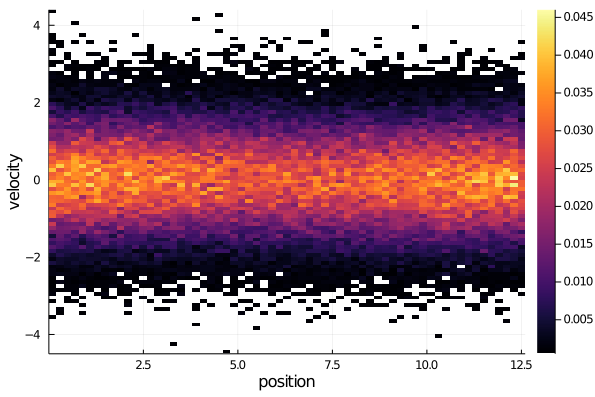
\includegraphics[width = \linewidth]{fig/kx=0.5, alpha=0.1, it=1.png}
\end{subfigure}
\begin{subfigure}{0.5\textwidth}
	\centering
	\caption{2s}
	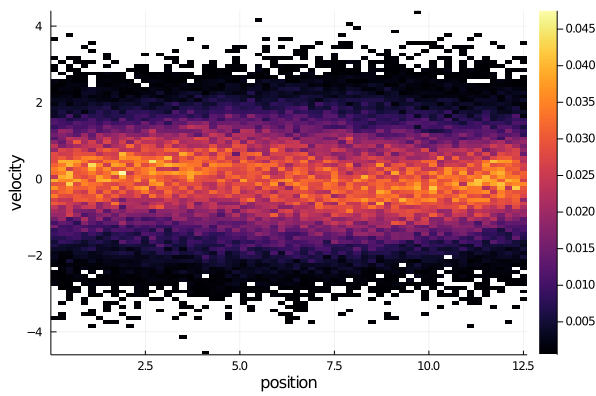
\includegraphics[width = \linewidth]{fig/kx=0.5, alpha=0.1, it=10.png}
\end{subfigure}

\begin{subfigure}{0.5\textwidth}
	\centering
	\caption{10s}
	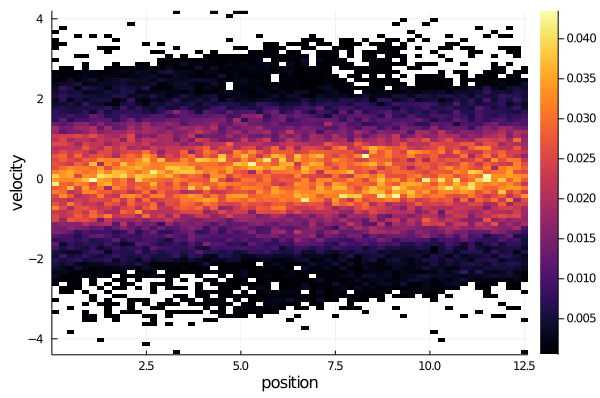
\includegraphics[width = \linewidth]{fig/kx=0.5, alpha=0.1, it=50.png}
\end{subfigure}
\begin{subfigure}{0.5\textwidth}
	\centering
	\caption{20s}
	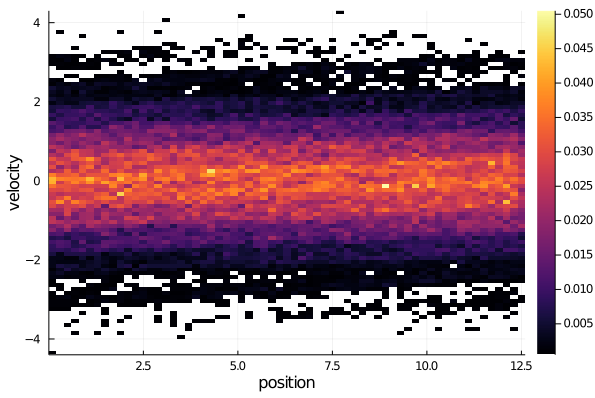
\includegraphics[width = \linewidth]{fig/kx=0.5, alpha=0.1, it=100.png}
\end{subfigure}
\end{figure}

La figure 1 représente la répartition des particules en position et vitesse pour kx = 0.5 et une perturbation initiale de $\alpha = 0.1$. L'ammortissement de Landau associé est en figure \ref{amort}. Sont représentées les trois méthodes de calcul de l'énergie vues précédement en traçant le logarithme néperien de la norme $L_2$ du champ électrique soit $\log(\sqrt{\int_{0}^{L} E^2(x,t) dx})$. On observe que la méthode PIC n'est plus efficace au delà de 15s alors que les deux autres méthodes donnent toujours des résultats cohérents. Cet effet est d'autant plus visible pour des petites perturbations comme sur les figures \ref{amort2} et \ref{amort3}, pour des valuers de $\alpha$ de 0.05 et 0.01.

\begin{figure}
	\centering
	\caption{Amortissement de Landau pour kx = 0.5, $\alpha = 0.1$}
	\label{amort2}
	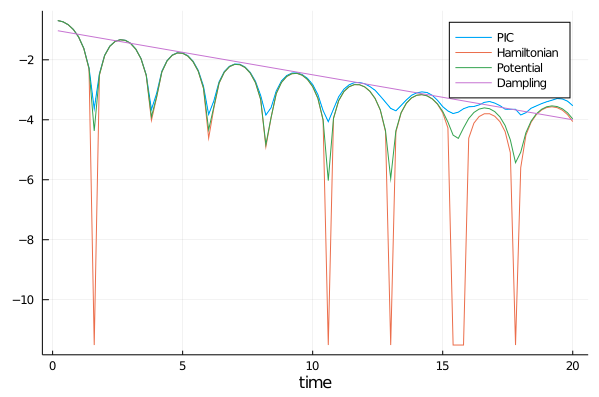
\includegraphics[width=\textwidth]{fig/kx=0.5, alpha=0.1, it=100, dampling.png}
\end{figure}

\begin{figure}
	\centering
	\caption{Amortissement de Landau pour kx = 0.5, $\alpha = 0.05$}
	\label{amort}
	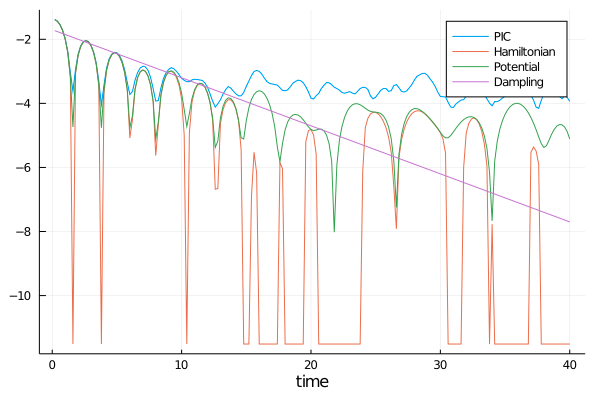
\includegraphics[width=\textwidth]{fig/kx=0.5, alpha=0.05, it=200, dampling.png}
\end{figure}

\begin{figure}
	\centering
	\caption{Amortissement de Landau pour kx = 0.4, $\alpha = 0.01$}
	\label{amort3}
	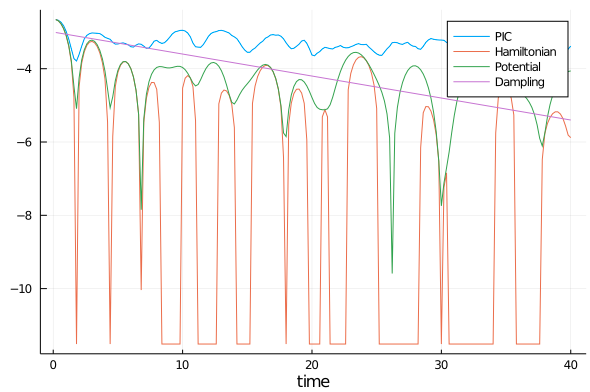
\includegraphics[width=\textwidth]{fig/kx=0.4, alpha=0.01, it=200, dampling.png}
\end{figure}

\end{document}